%
% ebenen.tex
%
% (c) 2018 Prof Dr Andreas Müller, Hochschule Rapperswil
%
\section{Ebenen}
\index{Ebene}
\index{Parameterdarstellung!einer Ebene}
\begin{figure}
\begin{center}
%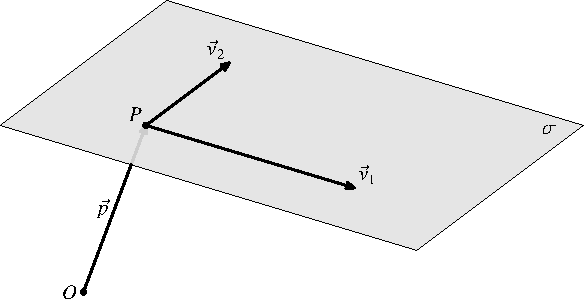
\includegraphics{images/v-8}
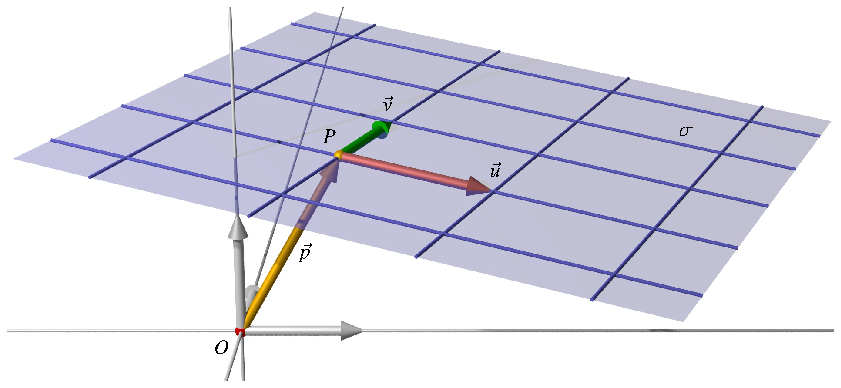
\includegraphics{3/images/ebene.pdf}
\end{center}
\caption{Parametrisierung einer Ebene mit Stüztvektor $\vec{p}$ und
Richtungsvektoren $\vec{u}$ und $\vec{v}$.
\label{image-parametrisierungebene}}
\end{figure}%
Ebenen zeichnen sich gegenüber Geraden dadurch aus, dass sich auf ihnen
ein Punkt nicht nur in einer Richtung, sondern unabhängig zwei Richtungen
bewegen kann.
Wir brauchen also einen zweiten Richtungsvektor und einen zweiten Parameter.
Die Punkte einer Ebene $\sigma$ werden also beschrieben durch
\[
\vec r=\vec p+t\vec v_1+s\vec v_2,
\]
(Abbildung~\ref{image-parametrisierungebene}).

\begin{beispiel}
Man finde die Parameterdarstellung der Ebene durch die Punkte
$A=(1,2,1)$,
$B=(3,4,-1)$ und
$C=(4,-1,0)$.

\smallskip

{\parindent 0pt Die} Vektoren $\vec u=\overrightarrow{AB}$ und
$\vec v=\overrightarrow{AC}$ können als Richtungsvektoren
verwendet werden, und ergeben als Parameterdarstellung:
\begin{equation}
\vec r=\begin{pmatrix}1\\2\\1 \end{pmatrix}
+
t\begin{pmatrix}2\\2\\-2\end{pmatrix}
+
s\begin{pmatrix}3\\-3\\-1\end{pmatrix}.
\label{beispielebene}
\end{equation}
\end{beispiel}

\subsection{Durchstosspunkt\label{subsection-durchstosspunkt}}
\index{Durchstosspunkt}
\begin{figure}
\begin{center}
%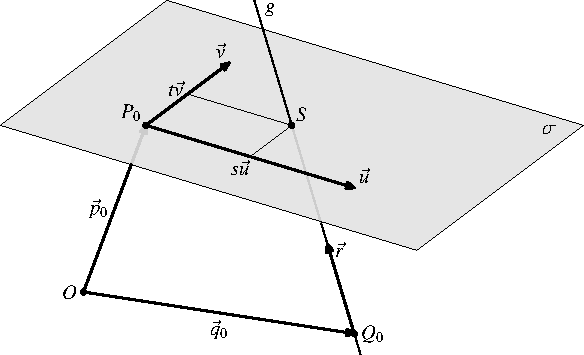
\includegraphics{images/v-9}
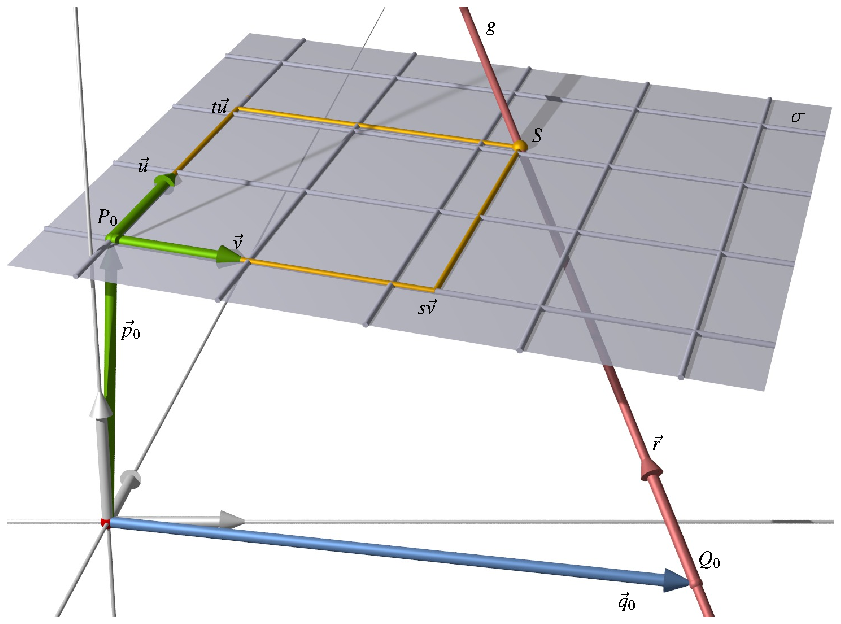
\includegraphics{3/images/durchstosspunkt.pdf}
\end{center}
\caption{Durchstosspunkt $S$ der Geraden $g$ durch die Ebene
$\sigma$.\label{image-durchstosspunkt}}
\end{figure}
Im dreidimensionalen Raum
sind eine Gerade $g$ und eine Ebene $\sigma$ je in Parameterdarstellung gegeben, also
\begin{align*}
\sigma&=
\{
\vec p_0+s\vec u+t\vec v\;
|\;s, t\in\mathbb R\}
\\
g&=
\{
\vec q_0+l\vec r\;
|\;l\in\mathbb R
\}
\end{align*}
Es soll der Durchstosspunkt $S$ der Gerade durch die Ebene gefunden
werden (Abbildung~\ref{image-durchstosspunkt}).
Dazu müssen wir die Parameterwerte für $s$, $t$ und $l$ finden,
für die gilt
\begin{align*}
\vec p_0+s\vec u+t\vec v
&=
\vec q_0+l\vec r
\\
s\vec u+t\vec v-l\vec r&=\vec q_0+\vec p_0
\end{align*}
Dies ist eine Vektorgleichung mit den drei Unbekannten $s$, $t$ und $l$,
sie entspricht drei linearen Gleichungen für diese Unbekannten.

Im Allgemeinen wird dieses Gleichungssystem genau eine Lösung haben,
nämlich den Durchstosspunkt.
Ist die Gerade parallel zur Ebene, hat das Gleichungssystem jedoch keine
Lösung, es gibt also auch keinen Durchstosspunkt.
Liegt die Gerade dagegen in der Ebene, gibt es unendlich viele Lösungen.

In den singulären Fällen ist es offenbar möglich, die Richtung $\vec r$
der Gerade durch die beiden Vektoren $\vec u$ und $\vec v$ in der Ebene
auszudrücken, die drei Vektoren $\vec u$, $\vec v$ und $\vec r$ sind
linear abhängig.

\begin{beispiel}
Finde den Durchstosspunkt der Geraden
\[
\vec r=
\begin{pmatrix} 5\\8\\3 \end{pmatrix}
+
l\begin{pmatrix} 1\\0\\1 \end{pmatrix}
\]
durch die Ebene (\ref{beispielebene}).

\smallskip

{\parindent0pt Zusammen} mit der Gleichung (\ref{beispielebene}) bekommen wir die
Vektorgleichung
\[
\begin{pmatrix}1\\2\\1 \end{pmatrix}
+
t\begin{pmatrix}2\\2\\-2\end{pmatrix}
+
s\begin{pmatrix}3\\-3\\-1\end{pmatrix}
=
\begin{pmatrix} 5\\8\\3 \end{pmatrix}
+
l\begin{pmatrix} 1\\0\\1 \end{pmatrix}
\quad\Rightarrow\quad
t\begin{pmatrix}2\\2\\-2\end{pmatrix}
+
s\begin{pmatrix}3\\-3\\-1\end{pmatrix}
+
l\begin{pmatrix} -1\\0\\-1 \end{pmatrix}
=
\begin{pmatrix} 4\\6\\2 \end{pmatrix}
\]
Das Gleichungssystem kann mit dem Gauss-Algorithmus
gelöst werden
\begin{align*}
\begin{tabular}{|>{$}c<{$}>{$}c<{$}>{$}c<{$}|>{$}c<{$}|}
\hline
 2%
\begin{picture}(0,0)
\color{red}\put(-3,4){\circle{12}}
\end{picture}%
& 3&-1&4\\
 2&-3& 0&6\\
-2%
\begin{picture}(0,0)
\color{blue}\drawline(-15,-2)(-15,24)(2,24)(2,-2)
\end{picture}
&-1&-1&2\\
\hline
\end{tabular}
&
\rightarrow
\begin{tabular}{|>{$}c<{$}>{$}c<{$}>{$}c<{$}|>{$}c<{$}|}
\hline
 1& \frac32&-\frac12&2\\
 0&-6%
\begin{picture}(0,0)
\color{red}\put(-7,3){\circle{15}}
\end{picture}%
& 1&2\\
 0& 2&-2&6\\
\hline
\end{tabular}
\rightarrow
\begin{tabular}{|>{$}c<{$}>{$}c<{$}>{$}c<{$}|>{$}c<{$}|}
\hline
 1& \frac32&-\frac12&2\\
 0& 1&-\frac16&-\frac13\\
 0& 0&-\frac53%
\begin{picture}(0,0)
\color{red}\put(-7,3){\circle{16}}
\end{picture}%
&\frac{20}3\\
\hline
\end{tabular}
\\
&
\rightarrow
\begin{tabular}{|>{$}c<{$}>{$}c<{$}>{$}c<{$}|>{$}c<{$}|}
\hline
 1& \frac32&-\frac12&2\\
 0& 1&-\frac16%
\begin{picture}(0,0)
\color{blue}\drawline(-15,24)(-15,-5)(2,-5)(2,24)
\end{picture}
&-\frac13\\
 0& 0& 1&-4\\
\hline
\end{tabular}
\rightarrow
\begin{tabular}{|>{$}c<{$}>{$}c<{$}>{$}c<{$}|>{$}c<{$}|}
\hline
 1& \frac32%
\begin{picture}(0,0)
\color{blue}\drawline(-8,10)(-8,-5)(2,-5)(2,10)
\end{picture}%
& 0&0\\
 0& 1& 0&-1\\
 0& 0& 1&-4\\
\hline
\end{tabular}
\\
&
\rightarrow
\begin{tabular}{|>{$}c<{$}>{$}c<{$}>{$}c<{$}|>{$}c<{$}|}
\hline
 1& 0& 0&\frac32\\
 0& 1& 0&-1\\
 0& 0& 1&-4\\
\hline
\end{tabular}
\end{align*}
Da $l=-4$ kann man jetzt den Durchstosspunkt berechnen, er ist $S=(1,8,-1)$.
\end{beispiel}

\subsection{Schnittgerade}
\index{Schnittgerade zweier Ebenen}
\begin{figure}
\begin{center}
%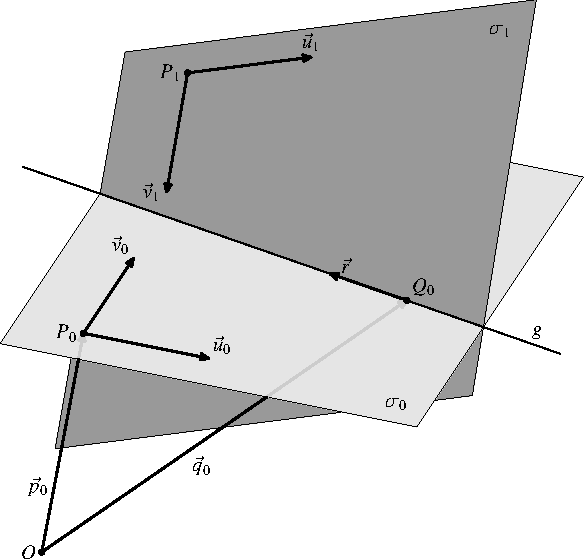
\includegraphics{images/v-10}
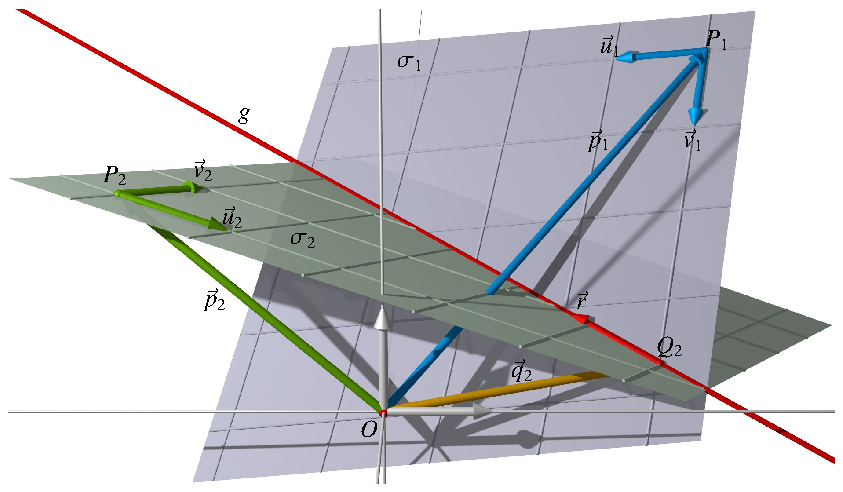
\includegraphics{3/images/schnittgerade.pdf}
\end{center}
\caption{Schnittgerade $g$ (rot) zweier Ebenen $\sigma_0$ (grün)
und $\sigma_1$ (blau).
\label{image-schnittgerade}}
\end{figure}
Im dreidimensionalen Raum sind zwei Ebenen
\begin{align*}
\sigma_0&=
\{\vec p_0+s_0\vec u_0+t_0\vec v_0\;|\;s_0, t_0\in\mathbb R\}
\\
\sigma_1&=
\{\vec p_1+s_1\vec u_1+t_1\vec v_1\;|\;s_1, t_1\in\mathbb R\}
\end{align*}
gegeben, gesucht ist deren Schnittgerade $g$
(Abbildung~\ref{image-schnittgerade}).
Diese besteht offenbar aus den Punkten, die sich für geeignete Parameterwerte
$s_0,t_0,s_1,t_1$ mit der Eigenschaft
\begin{align*}
p_0+s_0\vec u_0+t_0\vec v_0
&=
p_1+s_1\vec u_1+t_1\vec v_1
\\
s_0\vec u_0+t_0\vec v_0
-s_1\vec u_1-t_1\vec v_1
&=
-p_0+
p_1
\end{align*}
finden lassen.
Dies ist ein Gleichungssystem mit drei Gleichungen für
vier Unbekannte, im Allgemeinen wird sich also eine der Unbekannten
nicht bestimmen lassen, sondern die anderen Unbekannten werden sich
durch die vierte ausdrücken lassen.
Die Punkte der Schnittmenge sind also von der Form
\[
p_1+s_1(t_1)\vec u_1+t_1\vec v_1,
\]
wobei von der Form $s_1(t_1)=a+bt_1$ sein muss.
Setzt man dies ein, ergibt sich wieder eine Geradengleichung:
\[
p_1+s_1(t_1)\vec u_1+t_1\vec v_1
=
p_1+(a+bt_1)\vec u_1+t_1\vec v_1
=
(p_1+a\vec u_1)+t_1(b\vec u_1+v_1),
\]
eine Geradengleichung mit Richtungsvektor $\vec r = (b\vec u_1+v_1)$ und
Ausgangspunkt $\vec q_0=p_1+a\vec u_1$, also mit der Parametrisierung
\[
g=\{\vec q_0+t\vec r\;|\;t\in\mathbb R\}.
\]

\begin{beispiel}
Man finde die Schnittgerade der beiden Ebenen mit Parameterdarstellung
\[
\sigma_0:
\vec p_0+s_0\vec u_0+t_0\vec v_0
=\begin{pmatrix}5\\8\\6\end{pmatrix}
+s_0\begin{pmatrix}4\\6\\7\end{pmatrix}
+t_0\begin{pmatrix}2\\5\\6\end{pmatrix}
,
\qquad
\sigma_1:
\vec p_1+s_1\vec u_1+t_0\vec v_1
=\begin{pmatrix}5\\4\\4\end{pmatrix}
+s_1\begin{pmatrix}6\\6\\7\end{pmatrix}
+t_1\begin{pmatrix}5\\4\\4\end{pmatrix}
\]

\smallskip

{\parindent 0pt Wir setzen die beiden Parametrisierungen gleich und
erhalten}
\[
\begin{pmatrix}5\\8\\6\end{pmatrix}
+s_0\begin{pmatrix}4\\6\\7\end{pmatrix}
+t_0\begin{pmatrix}2\\5\\6\end{pmatrix}
=\begin{pmatrix}5\\4\\4\end{pmatrix}
+s_1\begin{pmatrix}6\\6\\7\end{pmatrix}
+t_1\begin{pmatrix}5\\4\\4\end{pmatrix}
\]
oder
\[
s_0\begin{pmatrix}4\\6\\7\end{pmatrix}
+t_0\begin{pmatrix}2\\5\\6\end{pmatrix}
-s_1\begin{pmatrix}6\\6\\7\end{pmatrix}
-t_1\begin{pmatrix}5\\4\\4\end{pmatrix}
=
\begin{pmatrix}0\\-4\\-2\end{pmatrix}
\]
Der Gauss-Algorithmus liefert für die Lösung das Tableau
\[
\begin{tabular}{|>{$}c<{$}>{$}c<{$}>{$}c<{$}>{$}c<{$}|>{$}c<{$}|}
\hline
4&2&-6&-5& 0\\
6&5&-6&-4&-4\\
7&6&-7&-4&-2\\
\hline
\end{tabular}
\rightarrow
\begin{tabular}{|>{$}c<{$}>{$}c<{$}>{$}c<{$}>{$}c<{$}|>{$}c<{$}|}
\hline
    1&   0&   0& -\frac{11}2& -26\\
    0&   1&   0&   4&  16\\
    0&   0&   1&  -\frac32& -12\\
\hline
\end{tabular}
\]
Die Variable $t_1$ ist frei wählbar, daraus lassen sich die anderen
Variablen bestimmen:
\[
\begin{linsys}{3}
s_0&=&-26&+&\frac{11}2t_1\\
t_0&=&16&-&4t_1\\
s_1&=&-12&+&\frac32t_1\\
\end{linsys}
\]
Setzt man dies in die ursprünglichen Ebenengleichungen ein, entsteht
die Parameterdarstellung der Schnittgeraden:
\begin{align*}
\begin{pmatrix}x\\y\\z\end{pmatrix}
&=
\begin{pmatrix}5\\8\\6\end{pmatrix}
+\biggl(-26+\frac{11}2t_1\biggr)\begin{pmatrix}4\\6\\7\end{pmatrix}
+(16-4t_1)\begin{pmatrix}2\\5\\6\end{pmatrix}
=
\begin{pmatrix}-67\\-68\\-80\end{pmatrix}
+t_1
\begin{pmatrix}14\\13\\\frac{29}2\end{pmatrix},\quad\text{oder}
\\
\begin{pmatrix}x\\y\\z\end{pmatrix}
&=
\begin{pmatrix}5\\4\\4\end{pmatrix}
+\biggl(-12+\frac32t_1\biggr)\begin{pmatrix}6\\6\\7\end{pmatrix}
+t_1\begin{pmatrix}5\\4\\4\end{pmatrix}
=
\begin{pmatrix}-67\\-68\\-80\end{pmatrix}
+t_1
\begin{pmatrix}14\\13\\\frac{29}2\end{pmatrix}
\end{align*}
Natürlich muss man in beiden Fällen die gleiche Gerade bekommen,
dies ist eine hübsche Kontrolle für die Richtigkeit des Resultates.
\end{beispiel}

\subsection{Vereinheitlichtes Lösungsverfahren\label{section-vereinheitlichtes-verfahren}}
Alle in den bisherigen Abschnitten vorgestellten Lösungsverfahren
laufen darauf hinaus, dass man für die Parameter der Parameterdarstellungen
Gleichungen dadurch aufstellt, dass man wo nötig Gleichungen herstellt.
Dies ist aber eigentlich ein unnötiger Schritt, den man auch dem
Gauss-Algorithmus überlassen könnte.

Traditionell wird das so gemacht, weil früher eine grosse Angst
davor bestand, auf grosse Gleichungssysteme zu stossen, deren Lösung
mühsam ist.
Diese Angst ist heute mit modernen Taschenrechnern und
Computer nicht mehr gerechtfertigt.

\subsubsection{Durchstosspunkt}
Um den Durchstosspunkt wie in \ref{subsection-durchstosspunkt} zu finden,
gehen wir wieder von den Parameterdarstellungen aus, schreiben jetzt
aber den gesuchten gemeinsamen Ortsvektor des Punktes
$({\color{red}x}, {\color{red}y}, {\color{red}z})$ explizit hin:
\[
\begin{pmatrix}
\color{red}x\\
\color{red}y\\
\color{red}z\\
\end{pmatrix}
=
\begin{pmatrix}1\\2\\1 \end{pmatrix}
+
{\color{red}t}\begin{pmatrix}2\\2\\-2\end{pmatrix}
+
{\color{red}s}\begin{pmatrix}3\\-3\\-1\end{pmatrix}
,\qquad
\begin{pmatrix}
\color{red}x\\
\color{red}y\\
\color{red}z\\
\end{pmatrix}
=
\begin{pmatrix} 5\\8\\3 \end{pmatrix}
+
{\color{red}l}\begin{pmatrix} 1\\0\\1 \end{pmatrix}
\]
Darin haben wir alle unbekannten Grössen {\color{red}rot} markiert.
Wir haben jetzt sechs Gleichungen mit sechs Unbekannten.
Der Gauss-Algorithmus liefert direkt die Lösung, sofern es eine gibt,
ohne dass man wie in Abschnitt \ref{subsection-durchstosspunkt}
die gefundenen Parameterwerte nochmals einsetzen müsste:
\[
\begin{tabular}{|>{$}c<{$}>{$}c<{$}>{$}c<{$}>{$}c<{$}>{$}c<{$}>{$}c<{$}|>{$}c<{$}|}
\hline
{\color{red}x}&
{\color{red}y}&
{\color{red}z}&
{\color{red}t}&
{\color{red}s}&
{\color{red}l}&\\
\hline
1&0&0&-2&-3& 0&1\\
0&1&0&-2& 3& 0&2\\
0&0&1& 2& 1& 0&1\\
1&0&0& 0& 0&-1&5\\
0&1&0& 0& 0& 0&8\\
0&0&1& 0& 0&-1&3\\
\hline
\end{tabular}
\rightarrow
\begin{tabular}{|>{$}c<{$}>{$}c<{$}>{$}c<{$}>{$}c<{$}>{$}c<{$}>{$}c<{$}|>{$}c<{$}|}
\hline
{\color{red}x}&
{\color{red}y}&
{\color{red}z}&
{\color{red}t}&
{\color{red}s}&
{\color{red}l}&\\
\hline
1&0&0&0&0&0&1\\
0&1&0&0&0&0&8\\
0&0&1&0&0&0&-1\\
0&0&0&1&0&0&1.5\\
0&0&0&0&1&0&-1\\
0&0&0&0&0&1&-4\\
\hline
\end{tabular}
\]
Daraus liest man einerseits den Durchstosspunkt $(1,8,-1)$ ab, andererseits
findet man die Parameterwerte, für die dieser Durchstosspunkt erreicht wird.

\subsubsection{Schnittgerade}
Die Schnittgerade der zwei Ebenen kann wie folgt gefunden werden.
Zunächst beschreiben wir mit der Parameterdarstellung, wie der
Ortsvektor eines beliebigen Punktes $(x,y,z)$ der Ebenen entsteht:
\[
\begin{pmatrix}
\color{red}x\\
\color{red}y\\
\color{red}z\\
\end{pmatrix}
=
\begin{pmatrix}5\\8\\6\end{pmatrix}
+{\color{red}s_0}\begin{pmatrix}4\\6\\7\end{pmatrix}
+{\color{red}t_0}\begin{pmatrix}2\\5\\6\end{pmatrix}
,\qquad
\begin{pmatrix}
\color{red}x\\
\color{red}y\\
\color{red}z\\
\end{pmatrix}
=
\begin{pmatrix}5\\4\\4\end{pmatrix}
+{\color{red}s_1}\begin{pmatrix}6\\6\\7\end{pmatrix}
+{\color{red}t_1}\begin{pmatrix}5\\4\\4\end{pmatrix}
\]
Hier hat man plötzlich 6 Gleichungen für 7 Unbekannte.
Wir erwarten also eine frei wählbare Variable, die dann als Parameter
für die Schnittgerade dienen kann.
Das Gausstableau ist
\[
\begin{tabular}{|>{$}c<{$}>{$}c<{$}>{$}c<{$}>{$}c<{$}>{$}c<{$}>{$}c<{$}>{$}c<{$}|>{$}c<{$}|}
\hline
{\color{red}x}&
{\color{red}y}&
{\color{red}z}&
{\color{red}s_0}&
{\color{red}t_0}&
{\color{red}s_1}&
{\color{red}t_1}&\\
\hline
1&0&0&-4&-2& 0& 0&5\\
0&1&0&-6&-5& 0& 0&8\\
0&0&1&-7&-6& 0& 0&6\\
1&0&0& 0& 0&-6&-5&5\\
0&1&0& 0& 0&-6&-4&4\\
0&0&1& 0& 0&-7&-4&4\\
\hline
\end{tabular}
\rightarrow
\begin{tabular}{|>{$}c<{$}>{$}c<{$}>{$}c<{$}>{$}c<{$}>{$}c<{$}>{$}c<{$}>{$}c<{$}|>{$}c<{$}|}
\hline
{\color{red}x}&
{\color{red}y}&
{\color{red}z}&
{\color{red}s_0}&
{\color{red}t_0}&
{\color{red}s_1}&
{\color{red}t_1}&\\
\hline
1&0&0&0&0&0&         - 14\phantom{.0}&-67\\
0&1&0&0&0&0&         - 13\phantom{.0}&-68\\
0&0&1&0&0&0&         - 14.5          &-80\\
0&0&0&1&0&0&-\phantom{0}5.5          &-26\\
0&0&0&0&1&0&\phantom{-0}4\phantom{.0}&\phantom{-}16\\
0&0&0&0&0&1&-\phantom{0}1.5          &-12\\
\hline
\end{tabular}
\]
Daraus liest man ab, dass es unendlich viele Punkte gibt, die auf beiden
Ebenen liegen, und dass $t_1$ als Parameter für die Geradengleichung
dienen kann.
Ausserdem kann man die Parameterdarstellung der Gerade ablesen:
\[
\begin{pmatrix}-67\\-68\\-80\end{pmatrix}
+t_1
\begin{pmatrix}14\\13\\14.5\end{pmatrix}.
\]




